\begin{prob}{002}{\hosi 1}{Daisu gakukon テンプレート問題}
四面体OABCは, $\mr{OA}=1, \mr{OB}=\mr{OC}=2$を満たし, 面$\mr{ABC}$が正三角形であるとする。
\ben
\item 正三角形$\mr{ABC}$の一辺の長さ$x$の取りうる値の範囲を求めよ。
\item 四面体OABCの体積の最大値を求めよ。
\een
\end{prob}

\subsection*{(1)}
簡単のため$x=2d$とおく。まず, 面$\mr{OAB}$の三辺は$1,2,2d$であり, この三辺について三角不等式が成り立つので
\beqn
\bcas
1<2+2d\\
2<1+2d\\
2d<1+2
\ecas
\quad \dou\quad \dfrac{1}{2} < d < \dfrac{3}{2}\quad \dou\quad 1<x<3　・・・\mbox{\maru{1}}
\eeqn
が必要。また, この範囲であれば面$\mr{OAC}, \mr{OBC}$に関しても三角不等式が成り立つ。\\
　次に, $\mr{BC}$の中点を$\mr{M}$とすると, $\mr{BM}=d, \mr{OM}=\sqrt{4-d^{2}}, \mr{AM}=\sqrt{3}d$である。点$\mr{A}$, 点$\mr{O}$はともに, $\mr{M}$を通る$\mr{BC}$に垂直な平面$p$上にある。一辺が$x=2d$のときにこの四面体が成り立つとするなら, $p$上で三角形$\mr{OAB}$が成り立つので, 三角不等式により
\beqn
\dfrac{1}{2}<d<\dfrac{3}{2}　かつ　
\bcas
\sqrt{3}d < 1+\sqrt{4-d^{2}}\\
1<\sqrt{3}d+\sqrt{4-d^{2}}\\
\sqrt{4-d^{2}} < \sqrt{3}d + 1
\ecas
\eeqn
を満たすことが必要。逆にこれを満たせば, 先に1辺$2d$の正三角形$\mr{ABC}$を与えて, $p$上の点$\mr{O}$であって, $\mr{OM}=\sqrt{4-d^{2}}$かつ$\mr{AM}=\sqrt{3}d$, したがって $\mr{OA}=1, \mr{OB}=\mr{OC}=2$を満たすようなものを取ることができる。 \\
　そこでこの不等式を解く。1式目と2式目は$(1-\sqrt{3}d)^{2} < 4-d^{2}$を考えることに同値。これを整理すると
\beqn
&& 4d^{2}- 2\sqrt{3}d -3 = x^2 - \sqrt{3}x - 3 <0\\
&\iff& \quad \dfrac{\sqrt{3}-\sqrt{15}}{2} < x < \dfrac{\sqrt{3}+\sqrt{15}}{2}　・・・\mbox{\maru{2}}
\eeqn
となる。3式目は, $\dfrac{1}{2}< d < \dfrac{3}{2}$のもとで両辺が正であるから, 二乗しても同値であり
\beqn
&& 4-d^{2} < (\sqrt{3}d + 1)^{2} \\
&\iff& 0<x^2 + \sqrt{3}x - 3\\
&\iff& x<\dfrac{-\sqrt{3} - \sqrt{15}}{2}\quad \mbox{or}\quad \dfrac{-\sqrt{3}+\sqrt{15}}{2}<x　・・・\mbox{\maru{3}}
\eeqn
である。以上\maru{1},\maru{2},\maru{3}を満たせば良いので, 求める範囲は
\begin{center}
\bolm{\dfrac{\sqrt{15}-\sqrt{3}}{2} < x  < \dfrac{\sqrt{15}+\sqrt{3}}{2}　　}
\end{center}
\subsection*{(2)}
$\angle{\mr{OAM}}=\theta$とおく。余弦定理により,
\[\cos{\theta} = \dfrac{1^{2}+(\sqrt{3}d)^{2} - (\sqrt{4-d^{2}})^{2}}{2\sqrt{3}d} = \dfrac{4d^{2} - 3}{2\sqrt{3}d}\]
なので,
\beqn
\sin^{2}{\theta} = 1- \left(\dfrac{4d^{2} - 3}{2\sqrt{3}d}\right)^{2} =\dfrac{1}{12d^{2}}\cdot (-16d^{4} + 36d^{2} - 9)
\eeqn
であり, $0<\theta<\pi$なので$\sin{\theta}>0$であるから,
\[\sin{\theta} = \dfrac{1}{2\sqrt{3}d}\sqrt{-16d^{4} + 36d^{2} - 9}\]
となる。$\mr{OA}=1$であるから, $\triangle{}\mr{OAM}$の$\mr{AM}$を底辺としたときの高さが$\sin{\theta}$である。$p$は$\mr{O}$を通り, 平面$\mr{ABC}$に垂直であるから, この高さは四面体の$\mr{ABC}$を底面とみたときの高さでもある。面$\mr{ABC}$の面積は$\sqrt{3}d^{2}$であるから, $\mr{AB}=x$のときの四面体の体積を$V(x)$とおくと
\beqn
V(x) &=& (\sqrt{3}d^{2})\times \dfrac{1}{2\sqrt{3}d}\sqrt{-16d^{4} + 36d^{2} - 9}  \times \dfrac{1}{3} \\
&=& \dfrac{1}{6} \sqrt{d^{2}(-16d^{4} + 36d^{2} - 9)}\\
&=& \dfrac{1}{12} \sqrt{x^{2}(-x^{4} + 9x^{2} - 9)}
\eeqn
$x^{2} = X$とおいて, $V(x) = \dfrac{1}{12}\sqrt{-X^{3} + 9X^{2} - 9X} $となる。\par
$W(X)=-X^{3} + 9X^{2} - 9X $とおくと,
\[W'(X) =-3(X^{2} - 6X +3) = -3\left( X-(3-\sqrt{6}) \right)\left(X- (3+\sqrt{6})\right)\]
となる。問(1)により, $X$の取る範囲は$\dfrac{9-3\sqrt{5}}{2} < X < \dfrac{9+3\sqrt{5}}{2}$であって, 数直線上で
\begin{center}
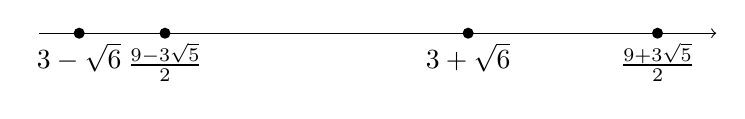
\begin{tikzpicture}
\draw[->] (0,0)--(8.6,0);
\fill (0.51,0) circle [radius=2pt] node [below=0pt] {$3-\sqrt{6}$};

\fill (1.6,0) circle [radius=2pt] node [below=0pt] {$\frac{9-3\sqrt{5}}{2}$};
\fill (5.45,0) circle [radius=2pt] node [below=0pt] {$3+\sqrt{6}$};

\fill (7.855,0) circle [radius=2pt] node [below=0pt] {$\frac{9+3\sqrt{5}}{2}$};
\end{tikzpicture}
\end{center}
と並ぶことに注意すると, 次の増減表を得る:
\begin{center}
$
\begin{array}{|c|*5{c|}}\hline
  X & \dfrac{9-3\sqrt{5}}{2} & \cdots  & 3+\sqrt{6} & \cdots  & \dfrac{9+3\sqrt{5}}{2} \\ \hline
  W'(x)&       &  + &   0    & - &      \\ \hline
  W(x) &    & \nea &  \mbox{極大}   &\sea &   \\ \hline
\end{array}
$
\end{center}
よって$V(x)=\dfrac{1}{12}\sqrt{W(X)}$も$X=3+\sqrt{6}$で最大となるので,
\beqn
&&(V(x)\mbox{の最大値}) \\
&=& \dfrac{1}{12}\sqrt{W(3+\sqrt{6})}\\
&=& \dfrac{1}{12}\sqrt{ -(3+\sqrt{6})\left\{ -(3+\sqrt{6})^{2} + 9(3+\sqrt{6}) - 9 \right\} }\\
&=& \dfrac{1}{12}\sqrt{-(3+\sqrt{6})\left\{3+3\sqrt{6} \right\}}\\
&=& \mbox{   \bolm{     \dfrac{\sqrt{3}}{12}\sqrt{9+4\sqrt{6}}  } }
\eeqn
